% Chapter 6
\section*{Preface}
In this chapter, performance of AIBs using two-dimensional (2D) materials was determined.
\pagebreak
\chapter{Aluminium batteries using various 2D materials as cathodes} 
\label{chap6} 

\section{Nano-structured molybdenum sulfide and selenide}

\subsection{Introduction}
Nano-sized materials increase the contact area between an electrode and electrolyte. The materials provide short path lengths for both ion diffusion and electron transport in comparison with bulk particles, which enhances the charge/ discharge rate. Since a short path length for electronic transport is created, materials having low electronic conductivity can also be utilised \cite{pitchai_nanostructured_2011}. The high surface area of the material allows large volume expansion/ contraction associated with ion transport and prevents cathode pulverisation leading to longer cycle-life \cite{zhang_ultrathin_2015, cong_intrinsic_2015}. 
Transition metal dichalcogenides (TMDs) have a large surface area and potential to undergo redox reactions. Nano TMDs have been widely explored as electrode materials since they have the potential to improve the electrochemical performance.  

\subsection{Experimental methods}
The materials were obtained from Tohoku university and used as received. 
%Before adding sulfur, pristine \ce{MoO3} (Wako chemicals) was ball-milled for 4 hours. 1 mmol of ascorbic acid (Wako chemicals) as a reducing agent was dissolved in 5 ml of water and the mixture was magnetically stirred for at least 20 minutes under air. Subsequently, 1 mmol of S powder (Sigma-Aldrich) and 0.3 mmol of ball-milled \ce{MoO3} were placed in the reactor. Lastly, 5 ml of ascorbic acid aqueous solution was injected into the reactor vessels containing the powder mixture. The sealed reactor was kept at 400$^{\circ}$C in a tube furnace for 30 minutes. After heating, the samples were collected in the same procedure as above.

\subsection{Results and discussion}
The Al/\ce{MoS2} cell delivered a specific capacity up to 55 mAh g$^{-1}$ based on the cathode loading of \ce{MoS2} (12 mg cm$^{-1}$) at a current density of 50 mA g$^{-1}$. The Al/\ce{MoSe2} achieved a  capacity of 65 mAh g$^{-1}$ at a similar current density. Figure \ref{Figures/chap6fig:MoX2YNCDCsCEs}a and b showed the charge and discharge curves with different current densities from 50 to 1500 mA g$^{-1}$ with cutoff voltages of 0.2 - 2.35 V. Figure \ref{Figures/chap6fig:MoX2YNCDCsCEs}c and d shows the rate performance of the Al/\ce{Mox2} cell. At higher charge–discharge rate, the cell showed decreased capacity and higher coulombic efficiency. At a high rate of 1500 mA g$^{-1}$, both Al/\ce{MoS2} and Al/\ce{MoSe2} cells could deliver a capacity of $\sim$20 mAh g$^{-1}$ and 99.5\% coulombic efficiency. The discharge capacity recovered to 50 mAh g$^{-1}$ when the rate slowed to 50 mA g$^{-1}$. Interestingly, no discharge voltage plateaus were observed for either cells. If we recall \ref{chap4} (Figure), bulk molybdenum dichalcogenides showed distinct voltage bends and plateaus. It seems no redox processes occurred in nano-structured \ce{MoS2} and \ce{ MoSe2}. Nevertheless, nano sized materials have very high surface area and the chloroaluminates can be adsorbed on their surface. Since the cell regains its initial capacity (>40 mAh g$^{-1}$) after charging and discharging at very high current rates (1500 mA g$^{-1}$), the adsorption appears to take place after every cycle.  

\begin{figure}[h!]
  \centering
  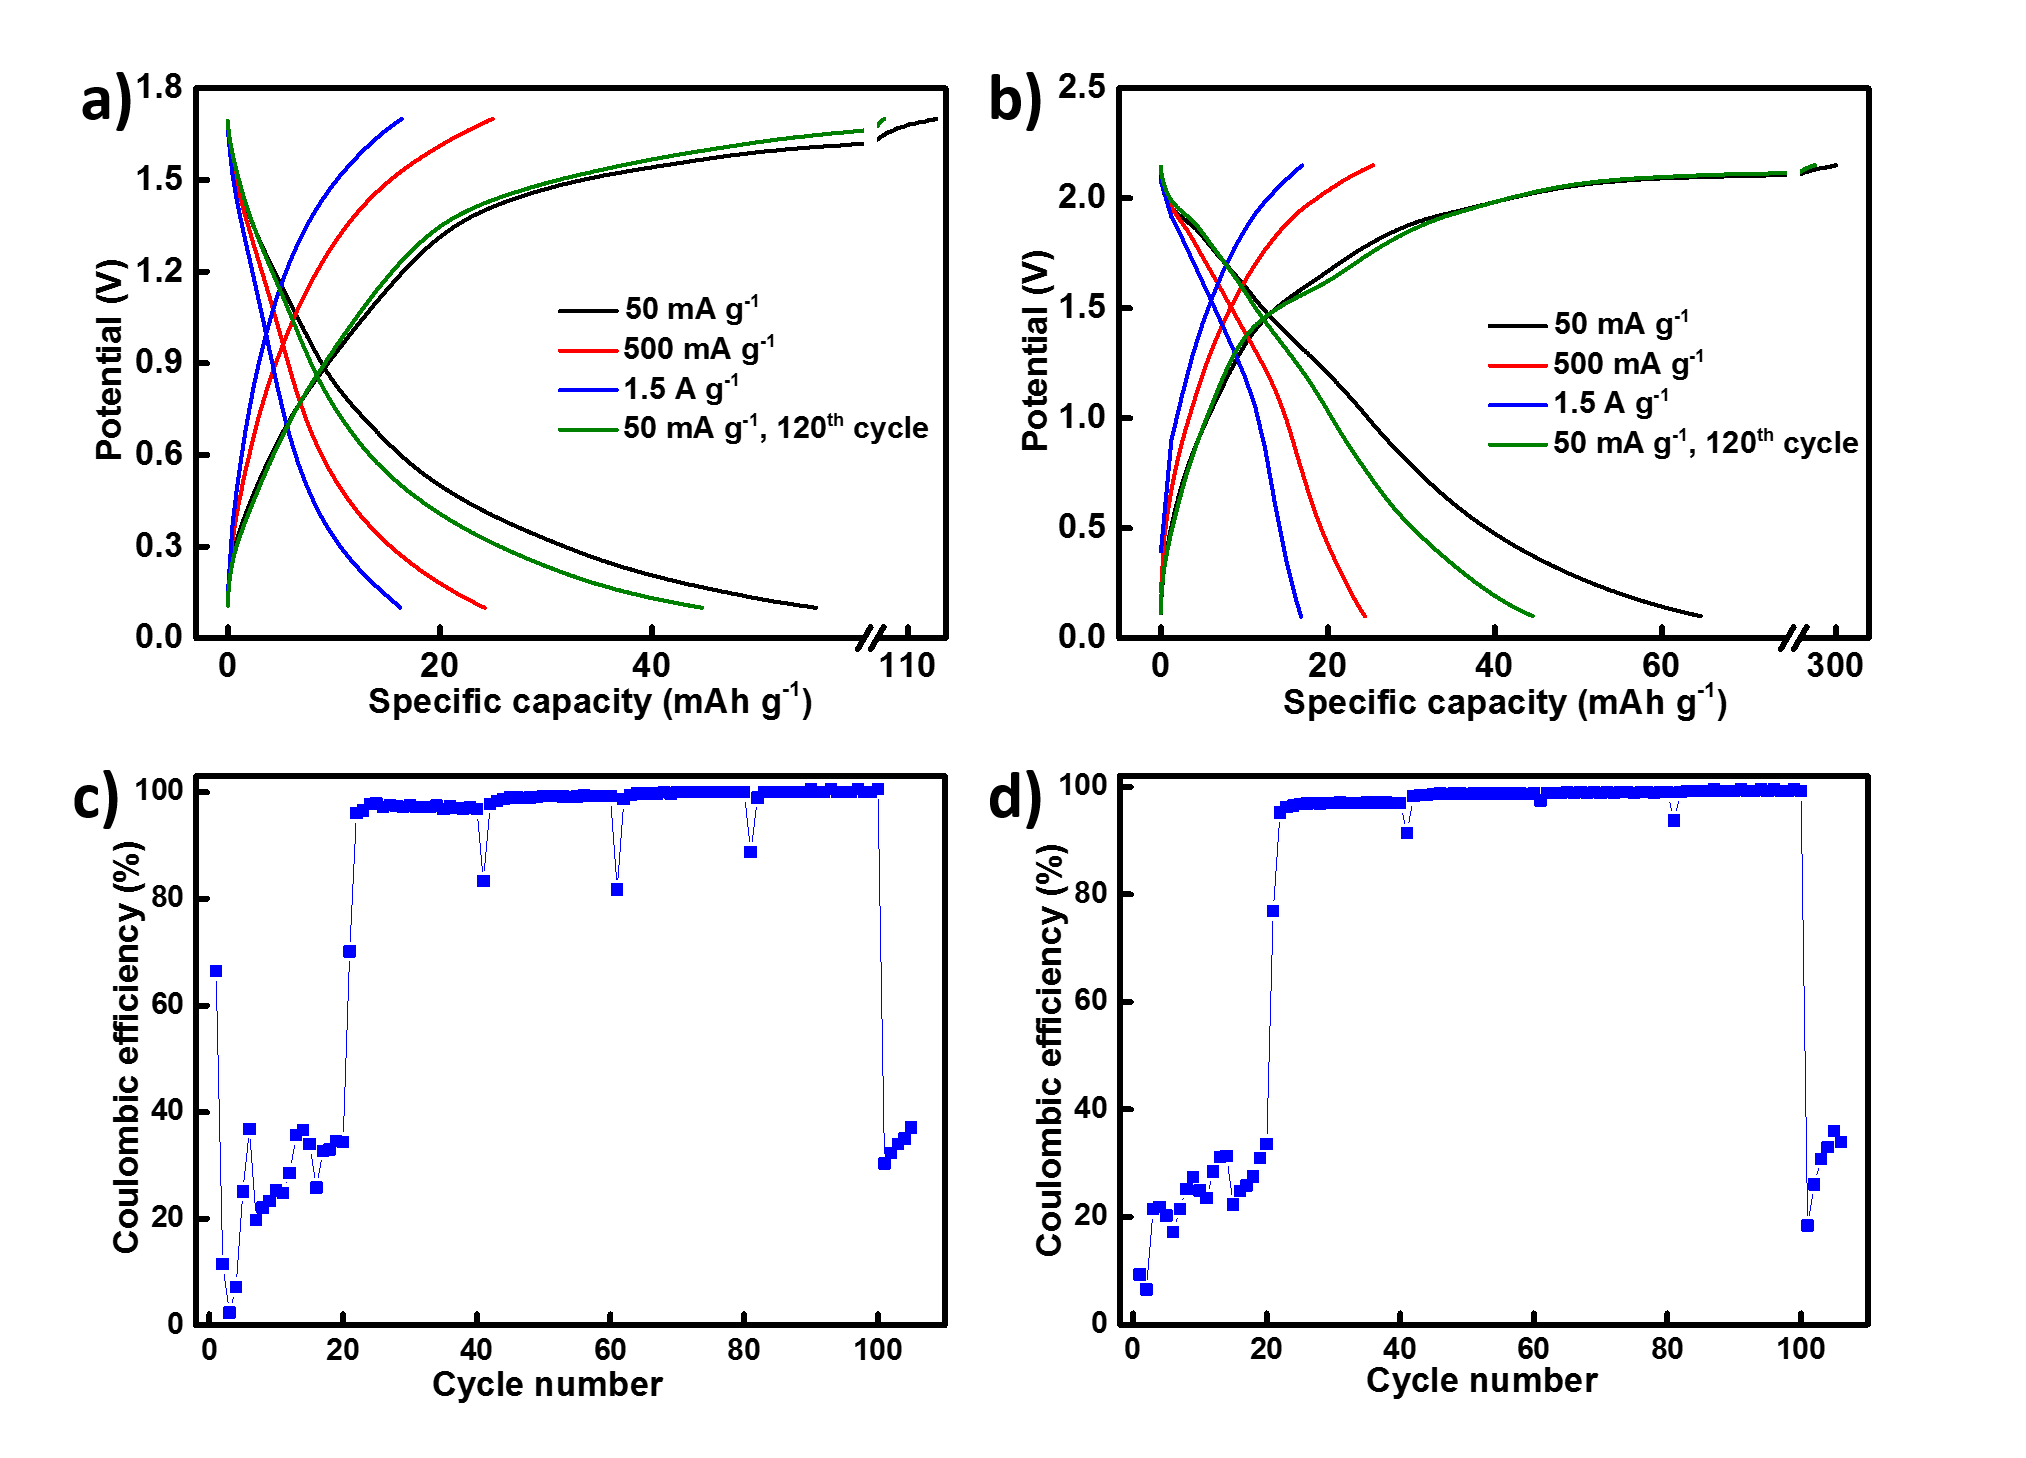
\includegraphics[width=\textwidth]{Figures/chap6fig/MoX2YNCDCsCEs}
    \caption{Galvanostatic charge and discharge curves of a) Al/\ce{MoS2} and b) \ce{MoSe2} cell at various current densities. Long-term stability test of c) Al/\ce{MoS2} and d) \ce{MoSe2} cells. All capacity was recorded between charging and discharging voltages of 0.2 and 2.35 V.}
  \label{Figures/chap6fig:MoX2YNCDCsCEs}
\end{figure}

\section{Tin oxide}

\subsection{Introduction}

\begin{figure}[th!]
  \centering
  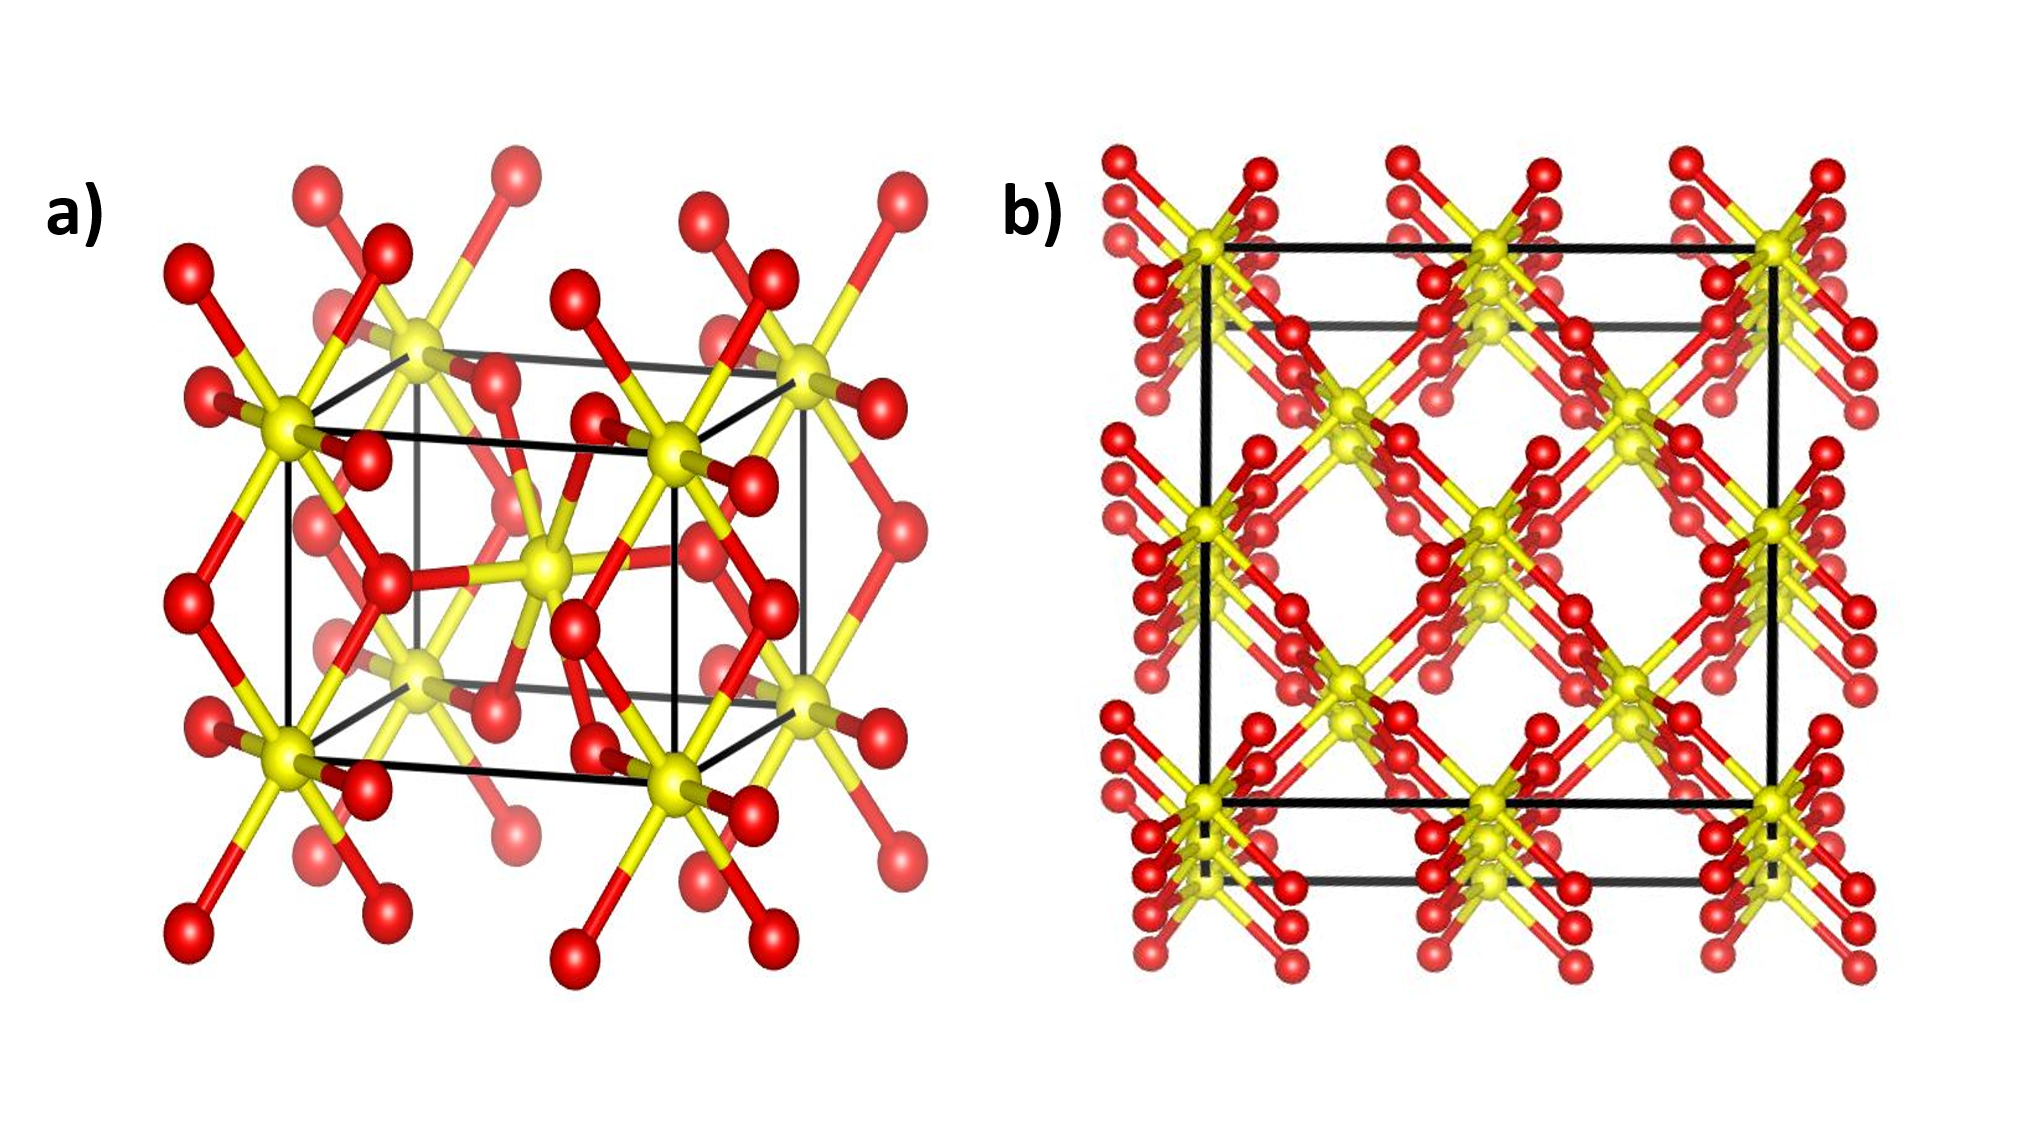
\includegraphics[width=\textwidth]{Figures/chap6fig/SnO2crys}
    \caption{Crystal structure of \ce{SnO2}. a) Tetragonal unit cell with space group P4/nmm and space group number 129. b) Top view of the crystal lattice.}
  \label{Figures/chap6fig:SnO2crys}
  \end{figure}
  
Tin, (Sn) has been a popular choice in energy storage devices due to its high conductivity and good thermal and mechanical stability. With high theoretical capacity of 992 mAh g$^{-1}$, it undergoes a reversible reaction in LIBs:

\begin{center}
    xLi + x\ce{e-} + ySn $\longleftrightarrow$ Li$_X$Sn  \cite{park_effect_2008}
\end{center}

However, it fails to deliver a steady performance. It undergoes high volumetric expansion during the lithiation process with a volume change of 200\%. Sn starts to aggregate leading to cathode pulverisation and capacity fades after a few cycles \cite{park_effect_2008, zhao_tin-based_2016}.  
Tin (+IV) oxide is an inorganic compound with the formula \ce{SnO2}. Due to its high theoretical capacity ($\approx$ 782mAh g$^{-1}$) and safe handling, \ce{SnO2} has an advantage over pure tin metal \cite{idota_tin-based_1997}. However, \ce{SnO2} underwent similar volumetric changes $\approx$ 300{\%}, which caused slow diffusion kinetics. After continuous charge-discharge cycles, cathodes experienced similar degradation and capacity faded.

 \begin{figure}[th!]
  \centering
  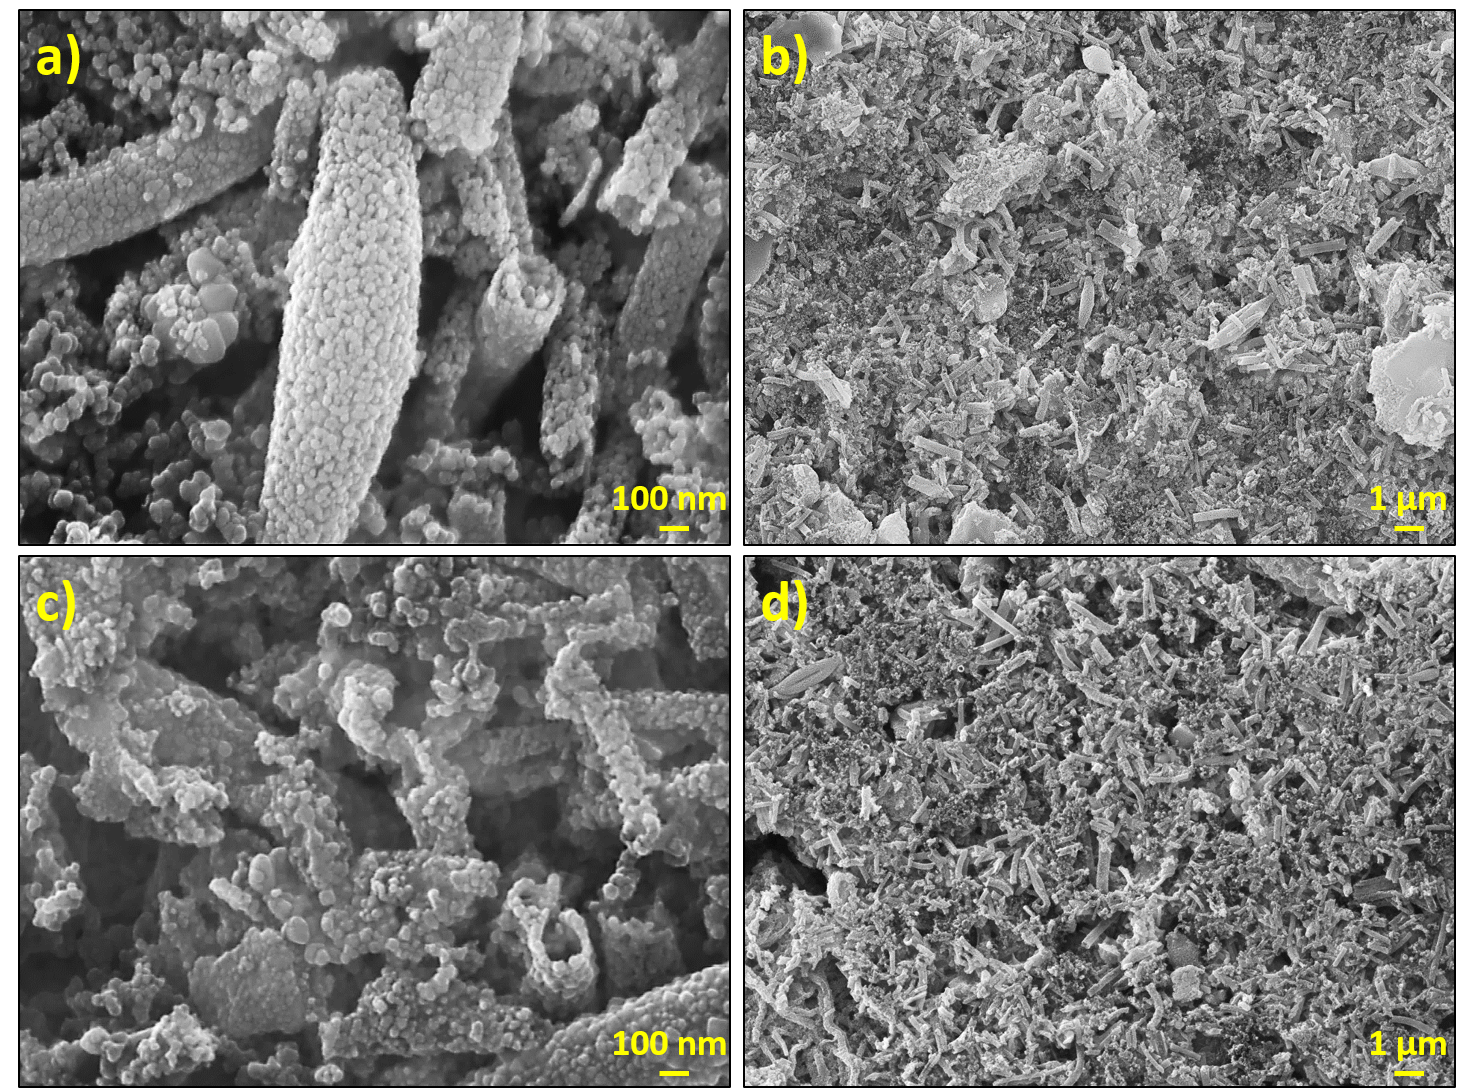
\includegraphics[width=\textwidth]{Figures/chap6fig/SnO2SEM}
    \caption{SEM images of a,c)pristine and b,d) cycled \ce{SnO2} cathode.}
  \label{Figures/chap6fig:SnO2SEM}
\end{figure}

% Lee \textit{et al.} obtained synthetic graphite modified by a highly dispersed \ce{SnO2} which improved the cell's performance . 
Adding carbonaceous materials to \ce{SnO2} seems to increase its surface area \cite{navarro-suarez_2d_nodate}. More active sites were now available for lithiation and the volume expansion/shrinkage was also controlled. Additionally, it improved the conductivity of the material \cite{nowak_composites_2018}. Several nano-structured tin-based materials such as nano-rods \cite{liu_direct_2009}, nano-belts \cite{duan_single_2005}, nano-wires \cite{huang_situ_2010}, nano-tubes \cite{wang_large-scale_2011} have been synthesised and a few have been tested as electrodes. Super-P is an additive that was used in making cathode slurries. It is conductive and amorphous carbon with an average particle size of 30-40 nm. 
Since intercalation of ions has been observed in AIBs (refer to \ref{chap4} and \ref{chap5}), electrospun \ce{SnO2} fibers were tested as cathodes in an aluminium-ion cell. 

\subsection{Experimental methods}
The material was obtained from University of Montpellier, France and was used as received. 

\subsection{Results and discussion}
To evaluate the electrochemical properties of the designed Al-ion cell, a galvanostatic discharge/charge reaction was performed at the cell voltage of 0.2-2.35 V at current densities ranging from 50-1500 mA g$^{-1}$. Figure \ref{Figures/chap6fig:SnO2perfCDC} displays the voltage vs. specific capacity plot of the AIB. The curves demonstrate a well defined discharge plateau at $\sim$ 0.55 V. In the first cycle, the
battery exhibited a capacity of >100 mAh g$^{-1}$ against 50 mAh g$^{-1}$ at the end of 120 cycles. The coulombic efficiency of the cell was not as high as would be needed for long-term practical use. It seems \ce{SnO2} undergoes similar  

 \begin{figure}[th!]
  \centering
  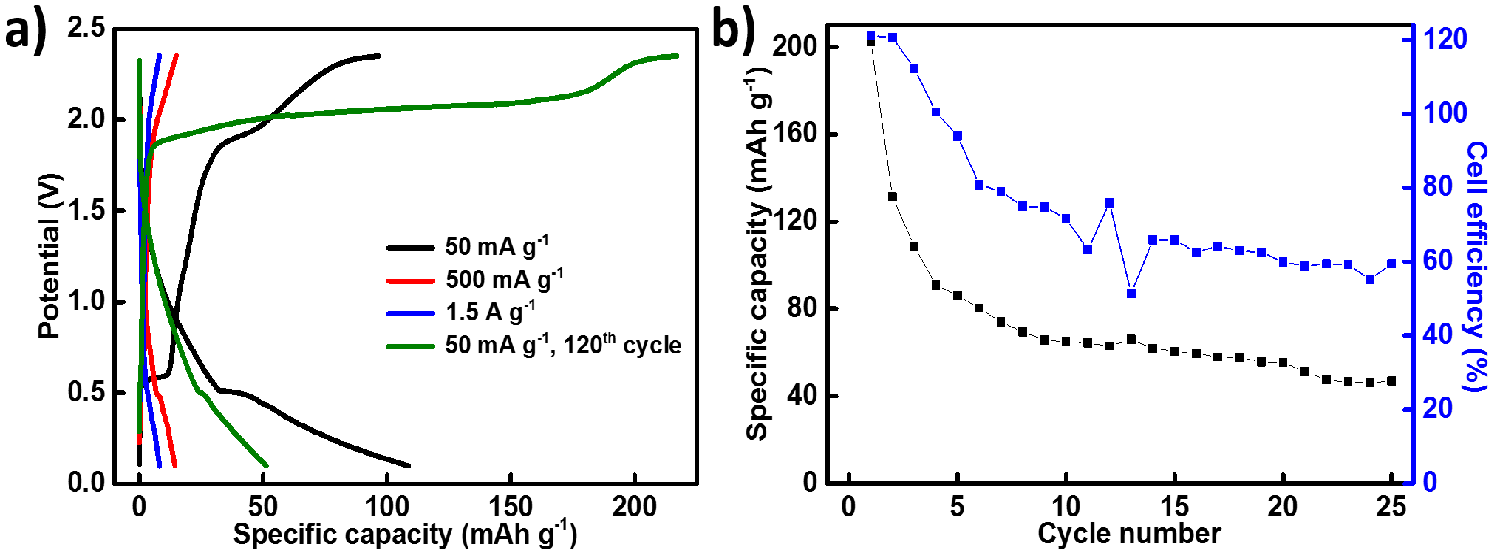
\includegraphics[width=\textwidth]{Figures/chap6fig/SnO2perfCDC}
    \caption{Galvanostatic charge and discharge curve of an Al/\ce{SnO2} cell at various current rates.}
  \label{Figures/chap6fig:SnO2perfCDC}
\end{figure}

 \begin{figure}[th!]
  \centering
  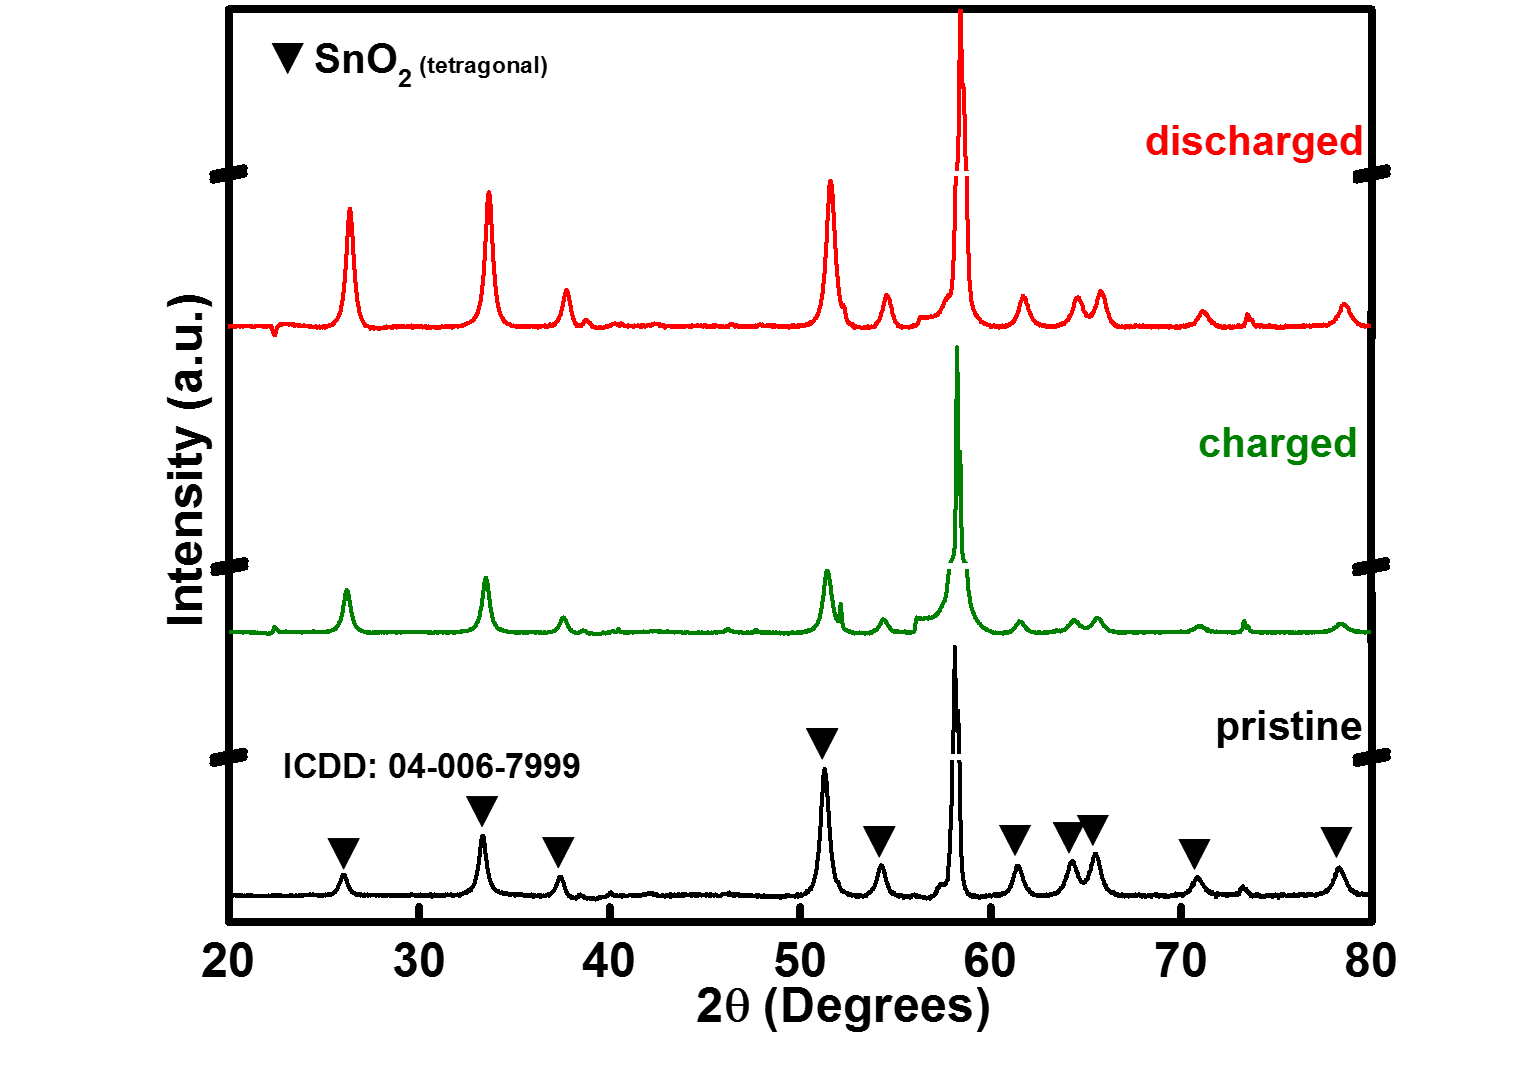
\includegraphics[width=\textwidth]{Figures/chap6fig/SnO2XRD}
    \caption{\textit{Ex-situ} X-ray diffraction patterns of \ce{SnO2} cathode in a pristine (black), charged (green) and discharged (red) state.}
  \label{Figures/chap6fig:SnO2XRD}
\end{figure}


\section{Molybdenum trioxide}

\subsection{Introduction}

 \begin{figure}[th!]
  \centering
  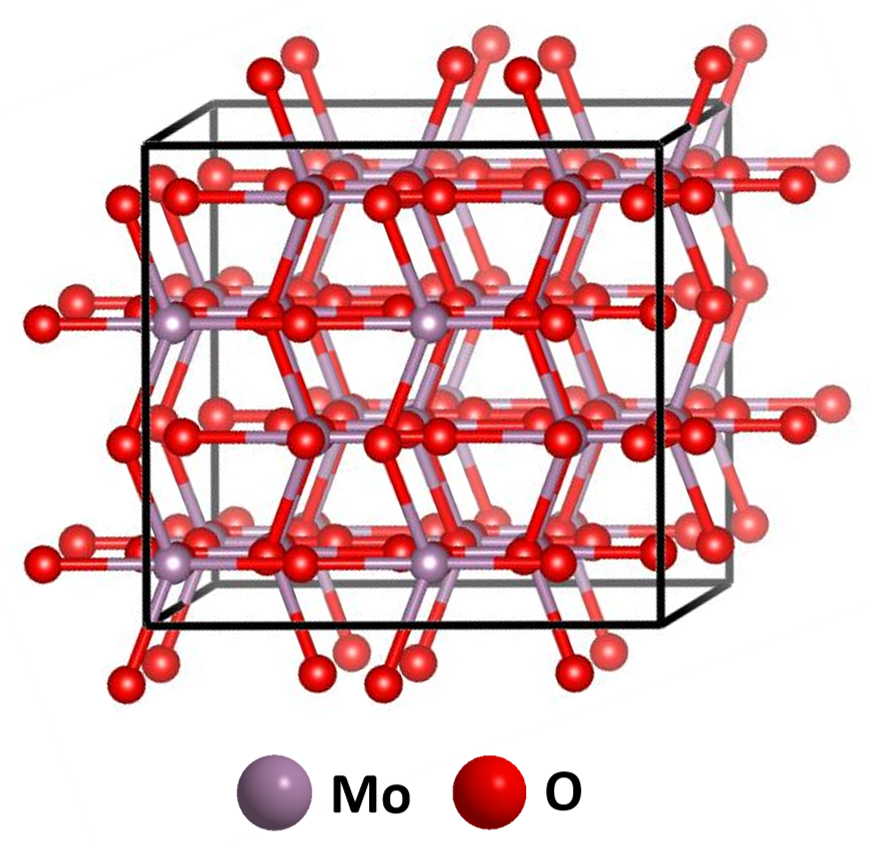
\includegraphics[width=\textwidth]{Figures/chap6fig/MoO3crys}
    \caption{Crystal structure of \ce{MoO3}. a) Tetragonal unit cell with space group P4/nmm and space group number 129. b) Top view of the crystal lattice.}
  \label{Figures/chap6fig:MoO3crys}
\end{figure}

Molybdenum trioxide, \ce{MoO3} is an intermediate formed during production of Mo metal. It consists of layers of \ce{MoO6} octahedra in an orthorhombic crystal held together by covalent forces and Van der Waals forces. Oxygen atoms in back and front of the chain link to other chains to build the layer. When used in lithium-ion, it sometimes undergoes a conversion reaction for lithium storage. High concentrations of unsolvated \ce{Li+} in the oxide host lattice cause significant irreversible morphological changes resulting in poor cell performance.
Since it has a structure with many interstitial sites and layers (Figure \ref{Figures/chap6fig:MoO3crys}, along with a \ce{Mo^{4+}}/\ce{Mo^{5+}} redox couple, it was important that we tested bulk \ce{MoO3} as a cathode material for aluminium-ion batteries.


\subsection{Experimental methods}
Molybdenum trioxide (\ce{MoO3} ACS reagent, $\geq$99.5\% was purchased from Sigma-Aldrich and used as received.

\subsection{Results and discussion}
At a high current density of 1500 mA g$^{-1}$ (Figure \ref{Figures/chap6fig:MoO3CDC}a), the \ce{MoO3} cathode afforded a  high specific capacity of $\sim$80 mAh g$^{-1}$ and coulombic efficiency a little above 100\%. After 120 cycles, the cathodic capacity was 75\% retained. Significantly, the charge/discharge curves throughout these cycles overlapped, demonstrating excellent reversibility of the \ce{MoO3} cathode. Constant specific discharge capacities, stable coulombic efficiency, and high average discharge voltage ($\sim$1.45 V) were illustrated within wide range of current densities from 50 mA g$^{-1}$ to 15000 mA g$^{-1}$. 

\begin{figure}[th!]
\centering
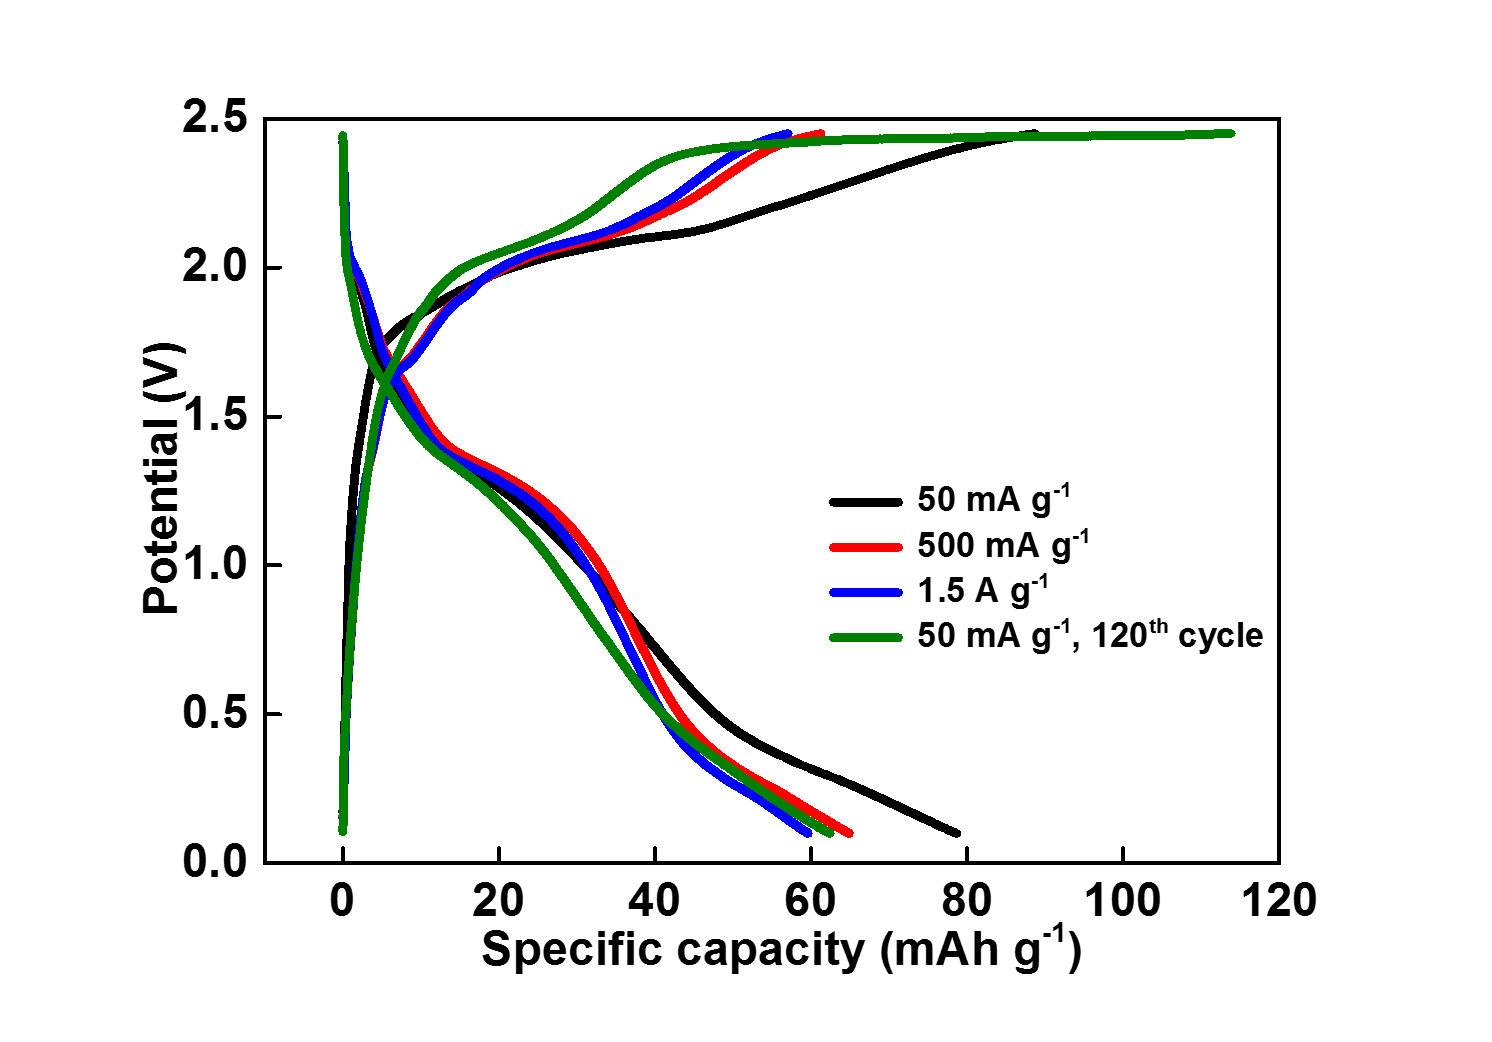
\includegraphics[width=\textwidth]{Figures/chap6fig/MoO3CDCredo}
\caption{Charge/discharge cycles of an Al/\ce{MoO3} cell at various current rates.}
\label{Figures/chap6fig:MoO3CDC}
\end{figure}

Notably, the cathode still retained a reversible high capacity of 60 mAh g$^{-1}$ at an extremely high current density of 1500 mA g$^{-1}$ with clear charging/discharging plateau. This reveals fast intercalation-based chemical redox reaction in the \ce{MoO3} cathode rather than physical adsorption-based electrical double-layer capacitive mechanism. These excellent electrochemical performances, especially high rate capability promise a new generation of energy storage system that can sustainably keep stable energy density of $\sim$85 Wh kg$^{-1}$.


\section{Graphitic Carbon Nitride}

\subsection{Introduction}

\begin{figure}[th!]
\centering
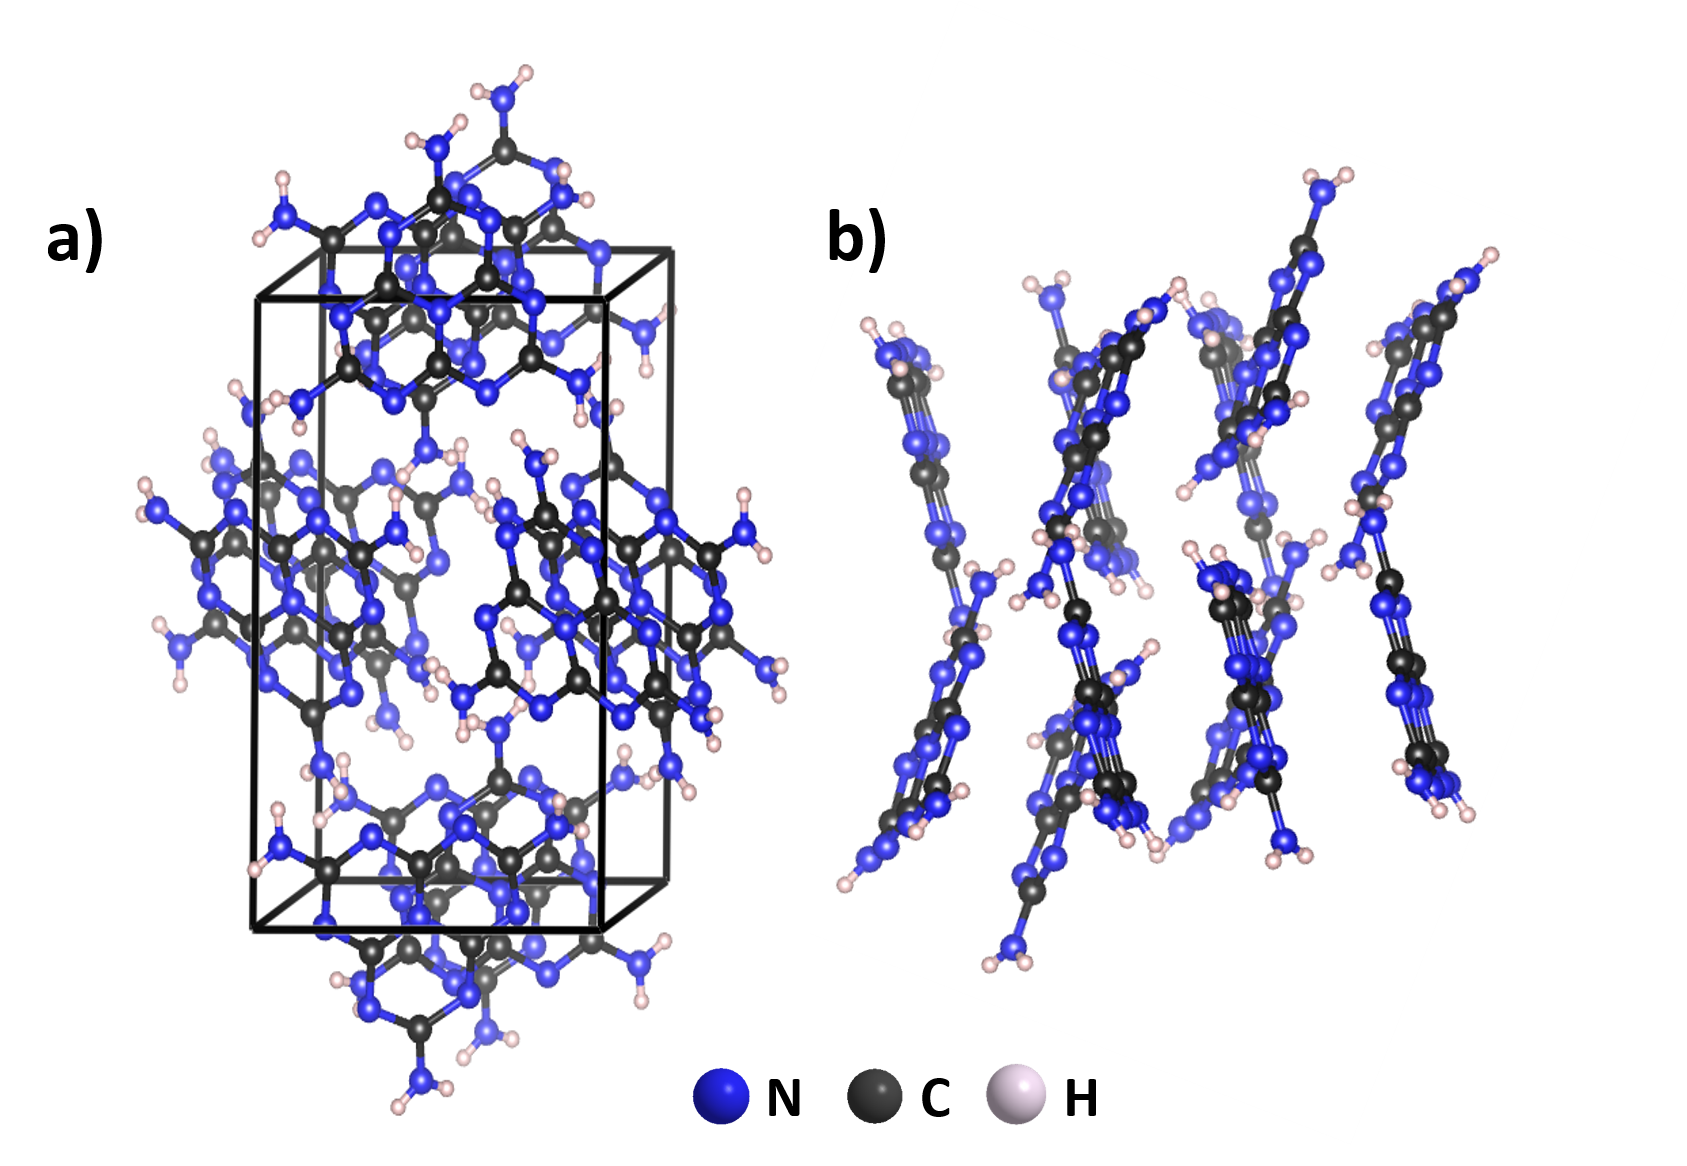
\includegraphics[width=\textwidth]{Figures/chap6fig/C3N4crys}
\caption{.}
\label{Figures/chap6fig:C3N4crys}
\end{figure}
\subsection{Experimental methods}
The material was obtained from the University of Auckland and was used as received. 

\subsection{Results and discussion}
Figure \ref{Figures/chap6fig:C3N4cdc} shows charge/discharge curves and charge/discharge capacities of the rechargeable Al cell with the \ce{C3N4} positive electrode at $\sim$80 mAh g$^{-1}$. The discharge capacity at the first cycle was 100 mAh g$^{-1}$, whereas that at the 120$^{th}$ cycle was below $\sim$80 mAh g$^{-1}$. Charge and discharge capacities were almost the same, suggesting that the rechargeable Al cell showed high coulombic efficiency. Figure \ref{Figures/chap6fig:C3N4cdc}a shows discharge capacities with different current densities. When discharge current was decreased to 50, capacity increased to 100 mAh g$^{-1}$, whereas at 1500 mA g$^{-1}$, capacity was below 20 mAh g$^{-1}$. In conclusion, \ce{C3N4} showed decent electrochemical activity for reversible ion intercalation and extraction with good cycle stability. 

\begin{figure}[th!]
\centering
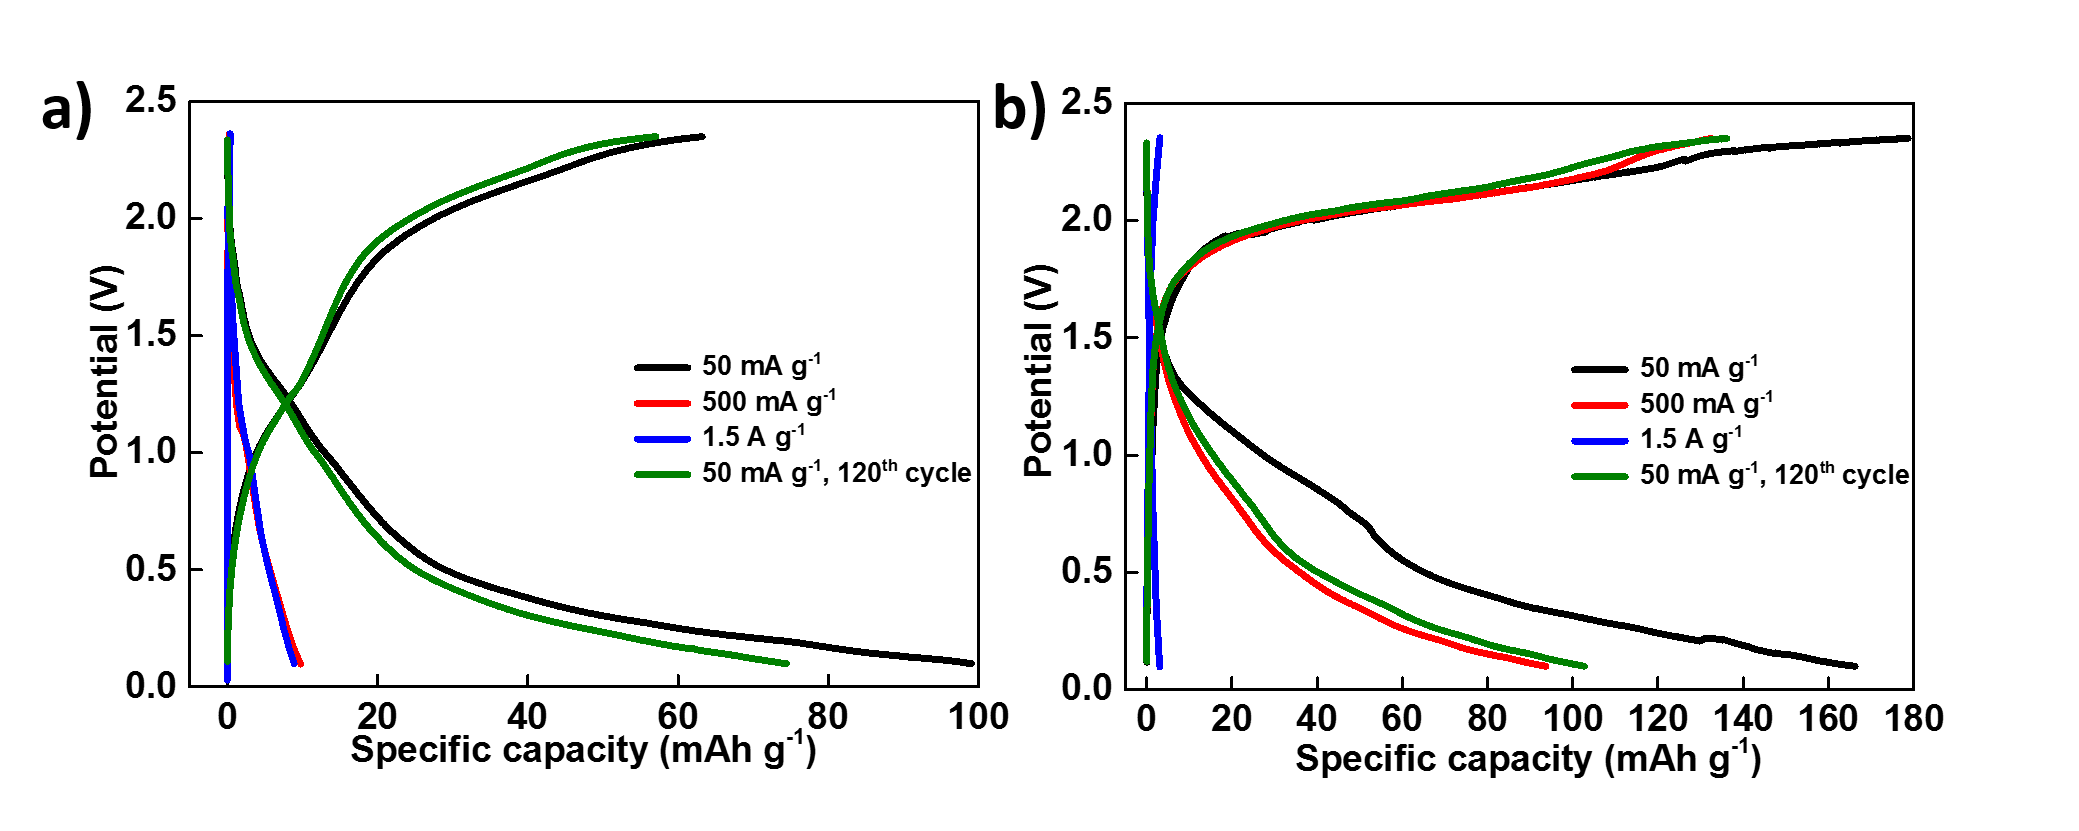
\includegraphics[width=\textwidth]{Figures/chap6fig/C3N4cdc}
\caption{Charge/discharge cycles of an Al/\ce{MoO3} cell at various current rates.}
\label{Figures/chap6fig:C3N4cdc}
\end{figure}

\section{Prussian blue}

\subsection{Introduction}

 \begin{figure}[tbh!]
  \centering
  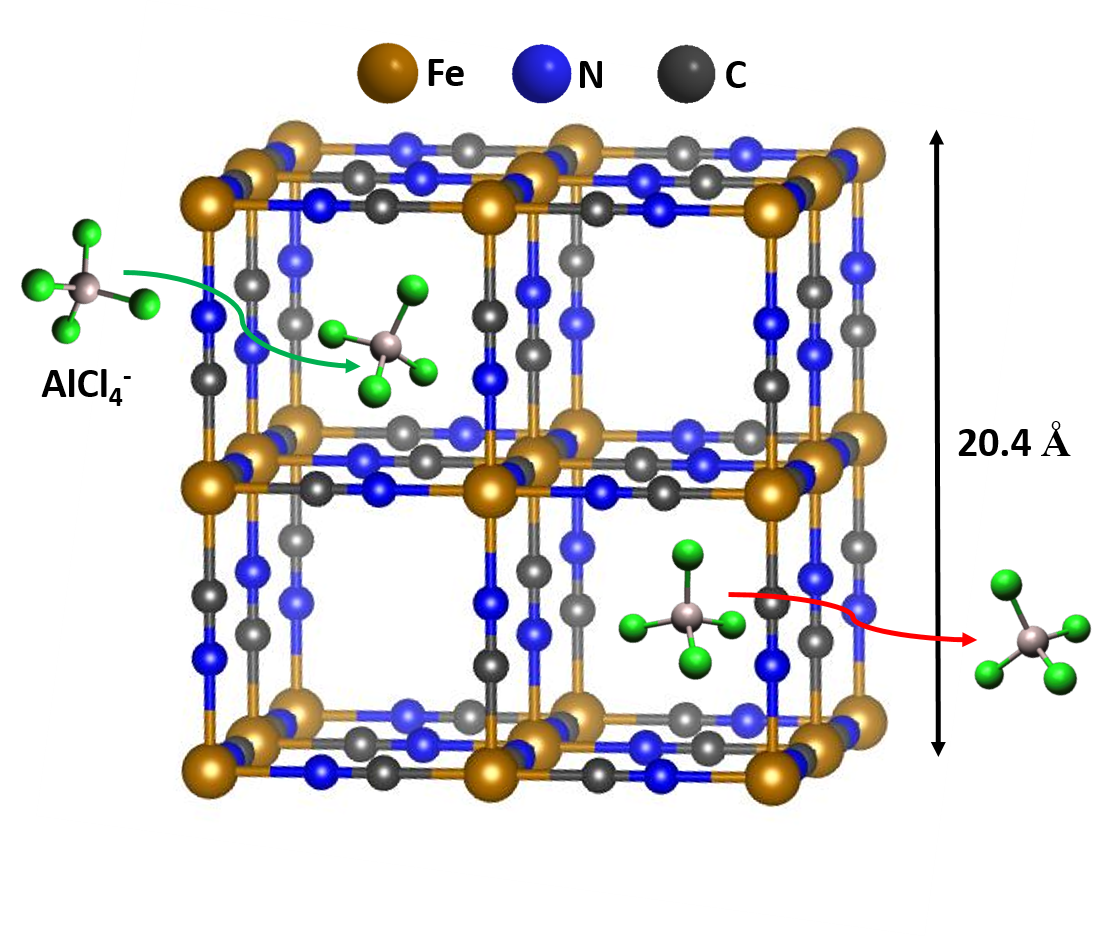
\includegraphics[width=\textwidth]{Figures/chap6fig/pbcrys}
    \caption{Crystal structure of prussian blue a) Tetragonal unit cell with space group P4/nmm and space group number 129. b) Top view of the crystal lattice.}
  \label{Figures/chap6fig:pbcrys}
\end{figure}

Prussian blue was originally commercialised in the dye industry. Since, it has been used for electrolysis, thermal power generation and energy storage. It has a face-centred cubic lattice with an open framework as shown in Figure \ref{Figures/chap6fig:pbcrys}, which helps in insertion of ions in the sub-cages. Its structure is very stable and has a number of redox sites present. Each molecular formula contains two redox centres \ce{M+2}/\ce{M3+}, where M is any transition metal (Fe, Co, Ni, Mn, Cu, Zn). It reaches 2\ce{e-} redox capacity after reversibly intercalating 2 monovalent alkali ions per molecular unit. Presence of large lattice interstices and ionic channels renders a high specific capacity. 

\subsection{Experimental methods}
\subsection{Results and discussion}
The first cycle galvanostatic charge–discharge curve of Al–prussian blue cells exhibited voltage plateaus at 1.8, 1.2 V and 0.6 V with a capacity of $\sim$140 mAh g. To investigate the rate capabilities of the battery, the cell was charged and discharged at various current densities (Figure \ref{Figures/chap6fig:pbCDC2}a) ranging from 50-1500 mA g$^{-1}$. the cycle performances and coulombic efficiency were investigated with a cut-off voltage between 2.35 V and 0.1 V at a current density of 50 mA g$^{-1}$ over 180 cycles, as shown in Figure \ref{Figures/chap6fig:pbCDC2}b. It can be seen that the capacity decreases significantly (45\%) over the first 20 cycles, Figure \ref{Figures/chap6fig:pbCDC2}b. The discharge capacity for the first cycle is 140 mAh g$^{-1}$, exhibiting multiple discharge voltage plateaus ranging from 1.9 V to 0.5 V. With the increase in current density, the capacity of the Al-ion battery gradually decreased to 5 mAh g$^{-1}$. It can be found that although capacities remained quite stable after initial cycling, coulombic efficiency showed a slightly decreasing trend, and decreased from 150 to $\sim$80\% after 180 cycles. 

 \begin{figure}[tbh!]
  \centering
  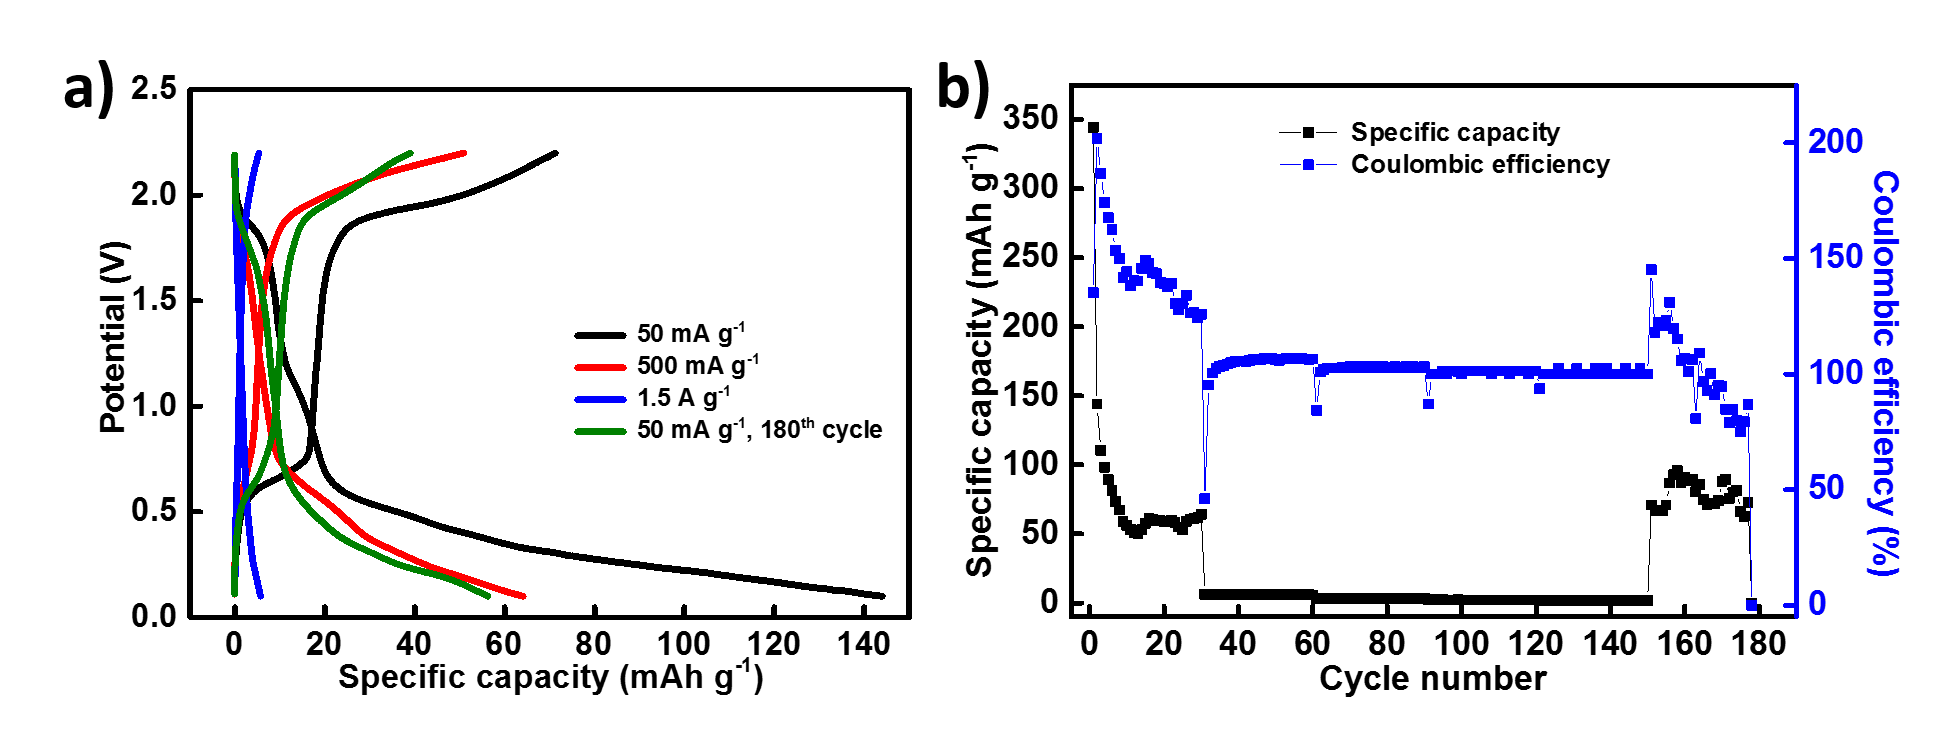
\includegraphics[width=\textwidth]{Figures/chap6fig/pbCDC2}
    \caption{Galvanostatic cycle test of an Al/\ce{C19Fe7N18} cell in a two-electrode setup at various current rates.}
  \label{Figures/chap6fig:pbCDC2}
\end{figure}

\subsection{Conclusion and future outlook}
Significant crystallography and voltammetry studies are underway to understand intercalation of aluminium into V2O5 and other layered oxides. These studies will help
shed light on the effect of variables such as the cell current
density and electrolyte formulation on the coulombic efficiency
and practical specific energy achievable in the Al-ion battery. As in the case of Li-ion secondary batteries, we anticipate significant opportunities for nanoscale engineering and chemical design of the Al-ion battery cathode to increase the overall cell potential. Additionally, we anticipate as significant efforts to pioneer ionic liquid and
